\documentclass[../thesis.tex]{subfiles}

\begin{document}

\section{Convolutional Neural Networks}

\subsection{Convolutional Neural Networks là gì?}

Convolutional Neural Network (CNN) là một kiến trúc mạng neurons giả định trước rằng dữ liệu đầu vào là dữ liệu ảnh, cho phép trích xuất các thuộc tính nhất định trong dữ liệu ảnh đó. Điều này khiến cho việc tính toán trở nên hiệu quả và giảm đáng kể số lượng tham số trong mạng \cite{cs231n}.

Không giống như các mạng neurons thông thường, các lớp của CNN gồm các neurons có dạng ma trận 3 chiều: chiều rộng (width), chiều cao (height), chiều sâu (depth). Có thể thấy rằng, các neurons trong một lớp chỉ kết nối với một vùng nhỏ của lớp phía trước nó \cite{cs231n}.
\begin{figure}[!htb]
	\begin{minipage}{0.48\textwidth}
		\centering
		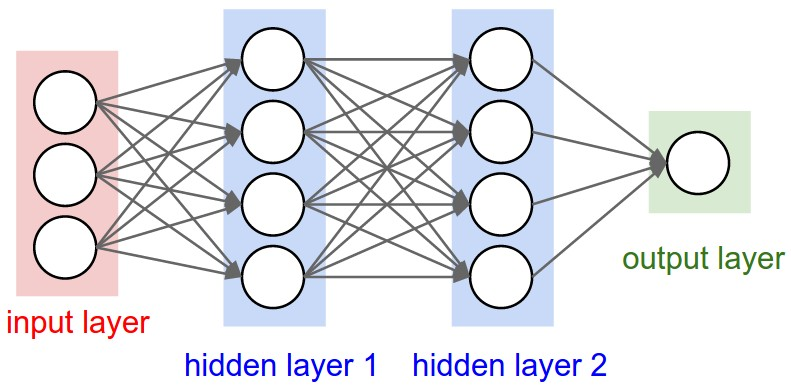
\includegraphics[width=.74\linewidth]{neural_net2.jpeg}
		\caption{Regular Neural Network}\label{Fig:NN}
	\end{minipage}\hfill
	\begin {minipage}{0.48\textwidth}
		\centering
		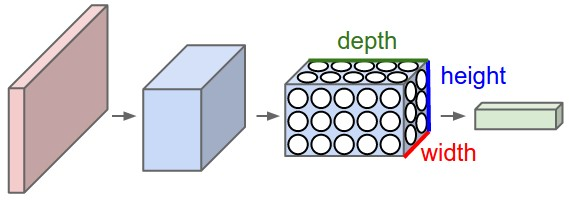
\includegraphics[width=\linewidth]{cnn.jpeg}
		\caption{Convolutional Neural Network}\label{Fig:CNN}
	\end{minipage}
\end{figure}

\subsection{Kiến trúc cơ bản của CNN}

Các mô hình CNN cơ bản thường bắt đầu bằng một conv layer và kết thúc bằng một (vài) fully connected layer. Ở giữa người ta thường chèn thêm các conv và pooling layer khác để tăng hiệu quả trích xuất các đặc trưng.

\begin{itemize}
  \begin{item}
	Lớp convolutional: là thành phần quan trọng nhất trong CNN. Mỗi neuron ở lớp này được xem như là một cửa sổ trượt, trượt trên ma trận đầu vào và thực hiện tính toán giá trị tích vô hướng tại mỗi vị trí mà cửa sổ này trượt qua. Các tham số quan trọng ở layer này là kernel size, padding(p) và stride (s). Kernel size là kích thước của cửa sổ trượt, được định nghĩa bằng chiều rộng (w), chiều cao (h) và chiều sâu (d) – chính là số neuron trong layer. Chiều rộng và chiều cao phải nhỏ hơn hoặc bằng chiều rộng(w*) và chiều cao(h*) của ma trận đầu vào. Stride định nghĩa khoảng cách của mỗi bước trượt, trong khi padding quyết định xem bao nhiêu dữ liệu 0 được chèn vào rìa của ma trận đầu vào. Kích thước đầu ra là $W \times H \times d$ với $W = \frac{w^*-w+2p}{s}+1$ và $H = \frac{h^*-h+2p}{s}+1$. Lớp convolutional thường sử dụng hàm kích hoạt ReLU cho feature map đầu ra.
	\begin{figure}[!htb]
		\centering
		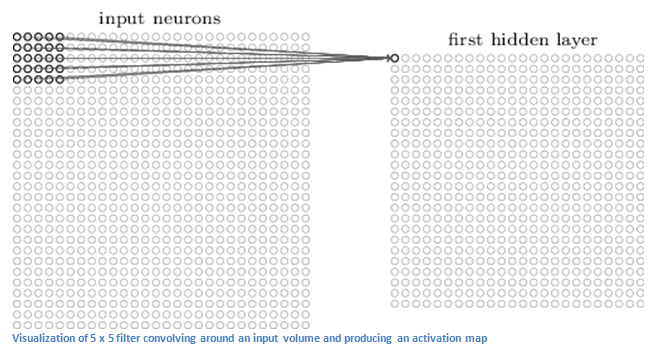
\includegraphics[width=\linewidth]{ActivationMap.png}
		\caption{Activation Map\cite{adeshpande3cnn1}}\label{activation_map}
	\end{figure}
  \end{item}
  
  \begin{item}
  Lớp pooling: thường nằm sau một convolutional layer để làm giảm kích cỡ cũng như các dữ liệu dư thừa của feature map. Một thuật toán pooling thường được sử dụng là max pooling. Max pooling sử dụng cửa sổ trượt trượt không trùng lắp qua ma trận đầu vào và chọn ra giá trị lớn nhất nằm trong cửa sổ để xây dựng ma trận đầu ra.
  \begin{figure}[!htb]
		\centering
		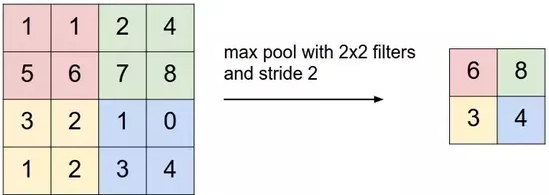
\includegraphics[width=\linewidth]{max_pooling.png}
		\caption{Max pooling}\label{max_pooling}
	\end{figure}
  \end{item} 
  \begin{item}
  Lớp dense (fully-connected): Thường thì có ít nhất 2 lớp dense nằm ở cuối cùng của mô hình CNN. Các lớp dense phía trước có nhiệm vụ làm phẳng (flatten) feature map trong khi lớp cuối cùng thực hiện việc predict bằng một mô hình regression.
  \end{item}
\end{itemize}

\begin{figure}[!htb]
	\begin{minipage}{0.48\textwidth}
		\centering
		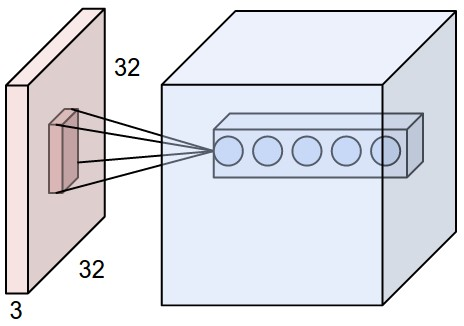
\includegraphics[width=.82\linewidth]{depthcol.jpeg}
		\caption{Một lớp convolutional}\label{Fig:depthcol}
	\end{minipage}\hfill
	\begin {minipage}{0.48\textwidth}
		\centering
		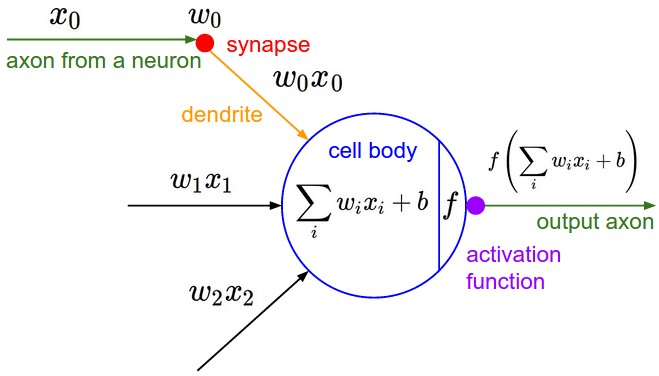
\includegraphics[width=\linewidth]{neuron_model.jpeg}
		\caption{Một neuron trong CNN}\label{Fig:neural_model}
	\end{minipage}
\end{figure}

\section{Region-based Convolutional Neural Networks}

Region-based Convolutional Neural Networks (R-CNN) là một mô hình nhận dạng vật thể (Object detection Model) do Ross Girshick, Jeff Donahue, Trevor Darrell và Jitendra Malik (UC Berkeley) đề xuất. Ý tưởng mô hình là với mỗi dữ liệu đầu vào, thực hiện trích xuất (extract) region proposals, trích xuất vector đặc trưng cho mỗi region, từ đó tiến hành việc phân lớp. Giai đoạn cuối cùng là hiệu chỉnh lại tọa độ của các region bằng một mô hình linear regression đơn giản.

\begin{figure}[!htb]
	\centering
	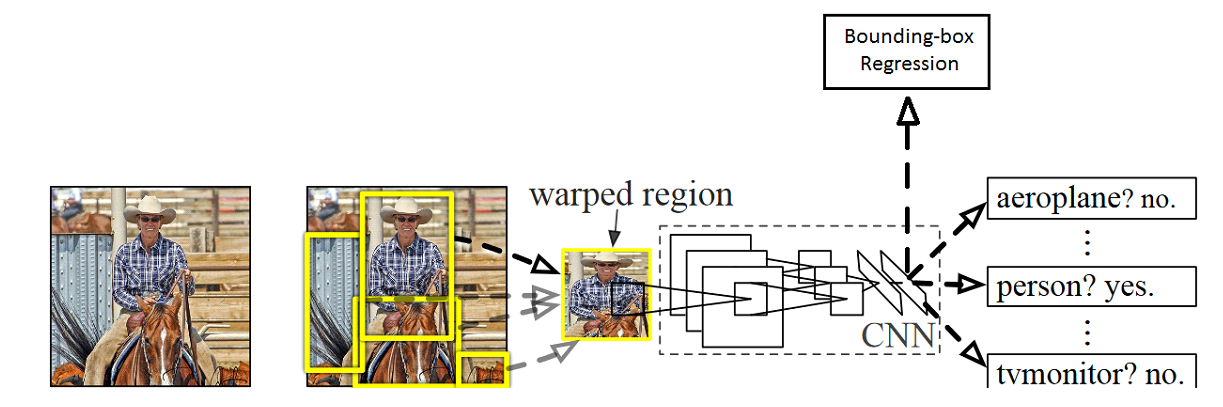
\includegraphics[width=\linewidth]{rcnn.PNG}
	\caption{Kiến trúc của R-CNN}\label{Fig:rcnn}
\end{figure}

\subsection{Selective search}

Kết hợp thế mạnh của Exhaustive search và Segmentation, Selective search giúp định vị vị trí của vật thể trong dữ liệu ảnh một cách hiệu quả. Đầu tiên, tập R gồm các initial region được khởi tạo. Tiếp đến, tính độ tương đồng (similarity) giữa các cặp region láng giềng. Các cặp region tương tự nhau nhất sẽ được gộp lại, đồng thời độ tương đồng sẽ được làm mới. Quá trình lặp đi lặp lại cho đến khi dữ liệu ảnh chỉ còn một region duy nhất.

\begin{figure}[!htb]
	\centering
	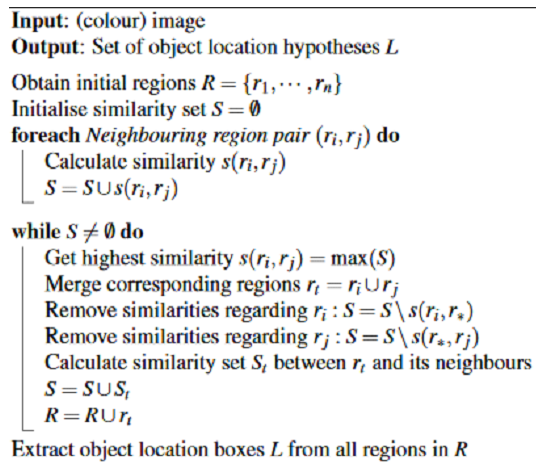
\includegraphics[width=0.65\linewidth]{selective-search.PNG}
	\caption{Pseudocode của selective search}\label{Fig:selective_search}
\end{figure}

Selective search được sử dụng trong giai đoạn trích xuất region proposal của mô hình R-CNN. Với mỗi dữ liệu ảnh, giải thuật thực hiện khoanh vùng 2000 region làm cơ sở cho việc trích xuất vector đặc trưng.

\begin{figure}[!htb]
	\centering
	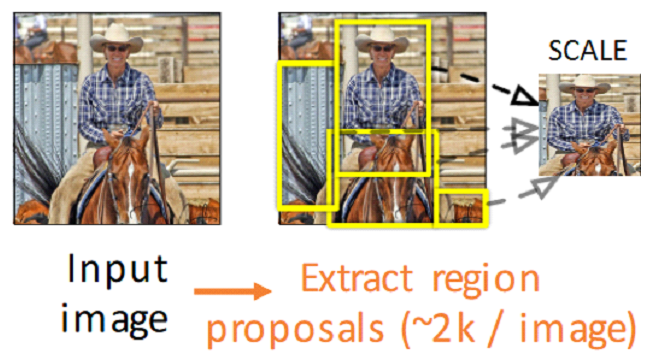
\includegraphics[width=0.65\linewidth]{rcnn_extract_reigions.PNG}
	\caption{Extract regions trong R-CNN}\label{Fig:rcnn_extract_regions}
\end{figure}

\subsection{Feature extraction}

Mỗi region sẽ được truyền thẳng (feed forward) qua một mạng CNN với nhiều lớp convolutional, pooling và fully connected. Vector đặc trưng sẽ được tính toán ra ở lớp fully connected gần với lớp output nhất.

\begin{figure}[!htb]
	\centering
	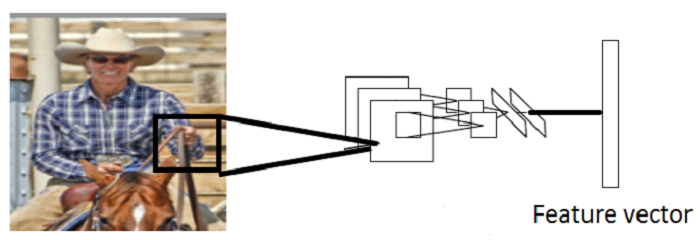
\includegraphics[width=0.65\linewidth]{features_extraction.PNG}
	\caption{Features extraction trong R-CNN}\label{Fig:rcnn_features_extraction}
\end{figure}

Để việc trích xuất đặc trưng có hiệu quả tốt, mạng CNN được huấn luyện với một tập dữ liệu lớn, sau đó thực hiện fine-tuning bằng các mẫu dữ liệu positive và negative được phân loại từ các region. Những region có tỷ lệ IoU\footnote{Intersection over union} với ground-truth box $\geq$ 0.5 sẽ được tính là positive, còn lại là negative.

\subsection{SVM classifiers}

Bộ phân lớp SVM có nhiệm vụ gắn nhãn cho các region. Việc huấn luyện các mô hình SVM diễn ra tương đối đơn giản:

\begin{itemize}
	\item Tạo các mẫu dữ liệu positive và negative. Positive được lấy từ ground-truth box, còn negative là các region có tỷ lệ IoU với ground-truth box < 0.3.
	\item Chọn ra các negative “khó” bằng phương pháp hard negative mining. Việc này giúp giảm bớt số lượng mẫu negative, đồng thời tăng hiệu quả huấn luyện.
	\item Tiến hành huấn luyện mô hình trên tập positive và negative. Tập dữ liệu trước tiên sẽ được trích xuất đặc trưng thông qua mạng CNN.
\end{itemize}

Ở giai đoạn predict, vector đặc trưng sẽ đi qua các bộ phân lớp SVM, từ đó nhãn tương ứng sẽ được gán.

\subsection{Bounding-box regression}

Sau khi đã phân lớp xong, vector đặc trưng được truyền qua một mô hình hồi quy tuyến tính để hiệu chỉnh vị trí của Bounding-box. Hàm lỗi của mô hình được định nghĩa như sau:

% TODO: Bổ sung phần loss function tại đây

\section{Fast R-CNN}

% TODO: Bổ sung phần này

\section{Faster R-CNN}

Fast R-CNN cải thiện thời gian thực thi và không gian lưu trữ bằng cách chia sẻ tính toán đối với hàng nghìn region. Tuy nhiên vẫn còn một tồn tại, đó là sự nghẽn cổ chai giữa quá trình trích xuất RoI và quá trình RoI Pooling. Các RoI được tạo ra bằng giải thuật Selective search, vốn không tận dụng được sức mạnh xử lý của GPU. Để giải quyết vấn đề trên, mô hình Faster R-CNN ra đời. Thay vì dùng các giải thuật truyền thống để trích xuất region proposal, Faster R-CNN thiết kế một mô hình CNN với tên gọi Region Proposal Network để thực hiện điều này.

\begin{figure}[!htb]
	\centering
	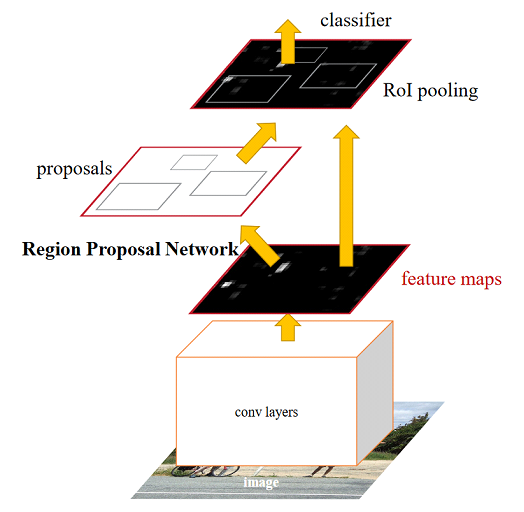
\includegraphics[width=0.65\linewidth]{faster-rcnn.PNG}
	\caption{Faster R-CNN}\label{Fig:faster_rcnn}
\end{figure}

\subsection{Region Proposal Network}

Region Proposal Network (RPN) nhận đầu vào là feature map của dữ liệu ảnh và xuất ra một tập các region proposal chứa các thông tin về nhãn[chú thích] và vị trí. Có thể hình dung RPN như một cửa sổ trượt. Cửa sổ này trượt qua từng location có kích thước  trên feature map và tính toán ra vector đặc trưng. Vector này được feed forward vào 2 lớp fully connected để dự đoán nhãn và vị trí.

\begin{figure}[!htb]
	\centering
	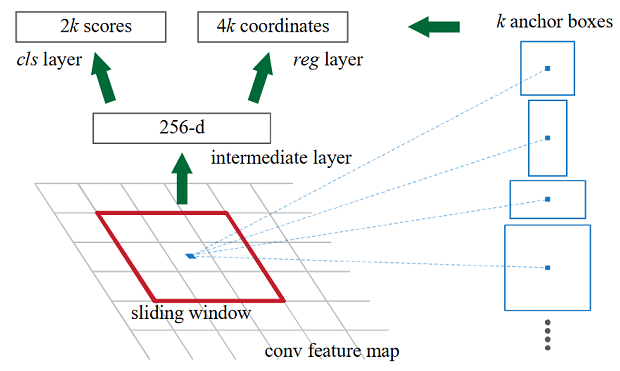
\includegraphics[width=0.65\linewidth]{rpn.PNG}
	\caption{Region Proposal Network}\label{Fig:rpn}
\end{figure}

\subsection{Anchor}

Tại mỗi location , có k anchor được tạo ra. Mỗi anchor được định nghĩa bởi tâm của location, scale và aspect ratio. Mặc định có 3 scale và 3 aspect ratio nên , tức là có 9 anchor (các anchor này cùng có chung một tâm).

\begin{figure}[!htb]
	\centering
	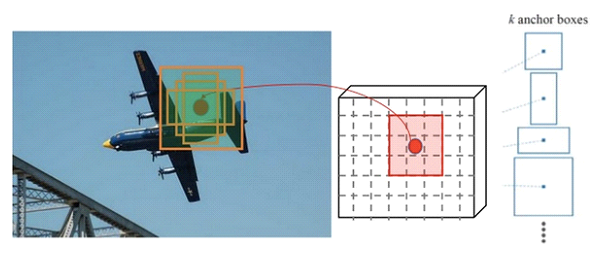
\includegraphics[width=0.65\linewidth]{anchors.PNG}
	\caption{Anchors}\label{Fig:anchors}
\end{figure}

\subsection{Loss function}

% TODO: Còn nữa

\end{document}